We next address the problem of \emph{unsupervised} learning. 
In this setting, we are not given any labeled data; all we get to see is a set of natural language sentences.  
The underlying question is: 
\begin{quote}
Can we learn something from raw text?
\end{quote}
This task is challenging, since the process by which linguistic structures are generated is not always clear; 
and even when it is, it is typically too complex to be
formally expressed. Nevertheless, unsupervised learning has been applied to a
wide range of NLP tasks, such as: 
\pos\ Induction  \citep{schutze1995distributional,merialdo1994tet,clark03combining},
Dependency Grammar Induction \citep{klein2004acl,smith2006annealing}, Constituency Grammar Induction \citep{klein2004acl}, Statistical Word Alignments 
\citep{brown94mathematic} and Anaphora Resolution \citep{charniak2009works}, just to name a few. 

Different motivations have pushed research in this area. From both a linguistic and cognitive point of view, 
unsupervised learning is useful as a tool to study language acquisition. 
From a machine learning point of view, unsupervised learning is a fertile ground for testing new learning methods, 
where significant improvements can yet be made. 
From a more pragmatic perspective, unsupervised learning is required
since annotated corpora is a scarce resource for different reasons. Independently of the reason, unsupervised learning is an increasing active field of research.

A first problem with unsupervised learning, since we don't observe any labeled data (i.e., 
the training set is now $\mathcal{D}_{U} = \{x^1,\ldots, x^M\}$), 
is that most of the methods studied so far (e.g., Perceptron, MIRA, SVMs) cannot be used since we cannot compare 
the true output with the predicted output. 
Note also that a direct minimization of the \emph{complete negative log-likelihood} of the data, $\log P_{\theta}(X^1=x^1,\ldots,X^M=x^m)$, 
is very challenging, since it would require marginalizing out (\emph{i.e.}, summing over) all possible hidden variables:
\begin{equation}
 \log P_{\theta}(X^1=x^1,\ldots,X^M=x^m) =  \sum_{m=1}^M \log \sum_{y \in \Lambda} P_{\theta} (X=x^m,Y=y).
\end{equation}
Note also that the objective above is \emph{non-convex} even for a linear model: hence, it may have local minima, which makes optimization much 
more difficult.%
%\footnote{Another observation is that normally we are restricted to generative models, 
%with some remarkable exceptions~\citep{smith2005acl}, since the objective of discriminative models when no labels are observed are 
%meaningless ($\sum_{y^m } P(y^m |x^m) = 1$); this rules out, for instance, Maximum Entropy classifiers.}

The most common optimization method in the presence of hidden (latent) variables is the Expectation Maximization (EM) algorithm, described in the next section. Note that this algorithm is a generic optimization routine that does not depend on a particular model. Later, in Section \ref{posi} we will apply the EM algorithm to the task of part-of-speech induction, where one is given raw text and a number of clusters and the task is to cluster words that behave similarly in a grammatical sense. 

\subsection{\label{em}Expectation Maximization Algorithm}
Given the training corpus $\mathcal{D}_{U} := \{x^1, \ldots, x^M\}$, training 
seeks model parameters $\theta$ that minimize the negative log-likelihood of the corpus:
\begin{equation}
\label{loglikelihoood}
\mathbf{Negative\;Log\;Likelihood\!:}\;\;\;\; \likelihood(\theta) = \widehat{\mathbb{E}} [-\log P_{\theta}(X)] = -\frac{1}{M}\sum_{m=1}^M \log \left( \sum_{y^m \in \Lambda} P_{\theta}(X=x^m,Y=y^m) \right),
\end{equation}
where $\widehat{\mathbb{E}}[f(X)] := \frac{1}{M}\sum_{m=1}^{M} f(x^m)$ denotes the empirical average of a function $f$ over the training corpus. Because of the hidden variables $y^1,\ldots,y^M$, the likelihood term contains a
sum over all possible hidden structures inside of a logarithm, which
makes this quantity hard to compute.

The most common minimization
algorithm to fit the model parameters in the presence of hidden
variables is the Expectation-Maximization (EM) algorithm. 
The EM procedure can be thought of intuitively in the following way. 
If we observe the hidden variables' values for all sentences in the
corpus, then we could easily compute the maximum likelihood value of
the parameters as described in Section \ref{ml}. 
On the other hand, if we had the model parameters we could label data
using the model, and collect the
sufficient statistics described in Section \ref{ml}.
However, since we are working in an unsupervised setting, we never get to
observe the hidden state sequence. Instead, given the 
training set $\mathcal{D}_{U} = \{x^1 \ldots x^M\}$, we will need to
collect \emph{expected} sufficient statistics (in this case, \emph{expected} counts) 
that
represent the number of times that each hidden variable is
expected to be used with the current parameters setting. These expected sufficient
statistics will then be used during learning as ``fake'' observations of
the hidden variables. Using the state and transition posterior distributions
described in Equations \ref{eq::nodePosterior} and \ref{eq::edgePosterior},
the expected sufficient statistics can 
be computed by the following formulas:

\begin{align}
\mathbf{Initial \ Counts\!:}\;\;\;\;  &  C_{\mathrm{init}}(c_k) = \sum_{m=1}^M
P_{\theta} (Y^m_1 = c_k \,\,|\,\, X^m = x^m); \label{eq::initialCountsPost}\\
%
%\mathbf{Final \ Counts\!:}\;\;\;\;  &  fc(\hv_l,\hv _m) = \sum_{\trex} 
%\Ind (\hs_N = \hv_l \mid \hs_{N-1} = \hv_m); \label{eq::finalCounts}\\
%
\mathbf{Transition \ Counts\!:}\;\;\;\;  &  C_{\mathrm{trans}}(c_k,c_l) =
\sum_{m=1}^M  \sum_{i = 2}^{N}
P_{\theta}(Y^m_i = c_k \wedge Y^m_{i-1} = c_l \,\,|\,\, X^m = x^m); \label{eq::transitionCountsPost}\\
%
\mathbf{Final \ Counts\!:}\;\;\;\;  &  C_{\mathrm{final}}(c_k) = \sum_{m=1}^M
P_{\theta} (Y^m_N = c_k \,\,|\,\, X^m = x^m); \label{eq::finalCountsPost}\\
%
\mathbf{Emission \ Counts\!:}\;\;\;\;  &  
C_{\mathrm{emiss}}(w_j,c_k) = \sum_{m=1}^M
\sum_{i = 1}^{N}
\Ind (x^m_i = w_j) P_{\theta}(Y^m_i = c_k \,\,|\,\, X^m = x^m); \label{eq::emissionCountsPost}
\end{align}

%\begin{align}
%\mathbf{Initial \ Counts\!:}\;\;\;\;  &  ic(\hv_l) = \sum_{d=1}^D
%\gamma_1 (\hv_l); \label{eq::initialCountsPost}\\
%\mathbf{Final \ Counts\!:}\;\;\;\;  &  fc(\hv_N,\hv _{N-1}) = \sum_{d=1}^D  \xi_{N-1} (\hv_l,\hv_m); \label{eq::finalCountsPost}\\
%\mathbf{Transition \ Counts\!:}\;\;\;\;  &  tc(\hv_l,\hv _m) = \sum_{d=1}^D \sum_{i = 1}^{N-1}  \xi_i (\hv_l,\hv_m); \label{eq::transitionCountsPost}\\
%\mathbf{State \ Counts\!:}\;\;\;\;  &  sc(\vv_q,\hv_m) = \sum_{d=1}^D \sum_{i = 1 , \obs_i = \vv_q }^{N}  \gamma_i (\hv_m). \label{eq::stateCountsPost}
%\end{align}

Compare the previous equations with the ones described in Section
\ref{ml} for the same quantities (Eqs.~\ref{eq::initialCounts}--\ref{eq::emissionCounts}). The main difference is that while in
the presence of supervised data you sum the observed events, when you
have no label data you sum the posterior probabilities of each
event. If these probabilities were such that the probability mass was
around single events then both equations will produce the same result.



The EM procedure starts with an initial guess for the parameters
$\theta^0$ at time $t = 0$. The algorithm keeps iterating 
until it converges to a local minima of the negative log likelihood. Each
iteration is divided into two steps:
\begin{itemize} 
 \item The {\bf{E-Step}} (Expectation) 
computes the posteriors for the hidden variables $P_{\theta^t}(Y|X=x^m)$
given the current parameter values $\theta^t$ and the observed variables $X=x^m$ for the $m$-th sentence. 
For an HMM, this can be done through the Forward-Backward algorithm described in the previous sections.
\item The {\bf{M-step}} (Maximization) uses those posteriors $P_{\theta^t}(Y|X=x^m)$ to
``softly fill in'' the values of the hidden variables $Y^m$, and
collects the sufficient statistics: initial counts (Eq: \ref{eq::initialCountsPost}), transition counts (Eq:
\ref{eq::transitionCountsPost}), 
final counts  (Eq: \ref{eq::finalCountsPost}),
and emission counts (Eq: \ref{eq::emissionCountsPost}). These
counts are then used to estimate maximum likelihood parameters $\theta^{t+1}$, as described in
Section \ref{ml}.
\end{itemize}

The EM algorithm is guaranteed to
converge to a local minimum of the negative log-likelihood $\likelihood(\theta)$, under mild
conditions.  
Note that we are not committing to the best assignment of the hidden variables, but
summing the occurrences of each parameter weighed by the posterior
probability of all possible assignments. 
This modular split into two intuitive and straightforward steps
accounts for the vast popularity of EM.%
\footnote{More formally, EM minimizes an \emph{upper bound} of $\likelihood(\theta)$ via block-coordinate descent. See \citet{Neal1998} for details. Also, even though we are presenting EM in the context of HMMs, this algorithm can be more broadly applied to any probabilistic model with latent variables.} %

% on an upper bound $F(q,\theta)$ using an auxiliary distribution over the latent variables
%$\auxq$:
%\begin{eqnarray}
%\likelihood(\theta)  &=& \XpD \left[-\log \sum_{\hseq}\joint \right]\\
%\label{eq:jensen}&=& \XpD \left[-\log \sum_{\hseq}
%\auxq*\frac{\joint}{\auxq}\right] \le \XpD \left[- \sum_{\hseq} \auxq\log \frac{\joint}{\auxq}\right] \\
%&=& \XpD \left[\sum_{\hseq} \auxq\log \frac{\auxq}{\joint}\right] =  F(q,\theta),
%\end{eqnarray}
%where we have multiplied and divided the $\joint$ by the same quantity
%$\auxq$, and 
%the lower bound comes from applying Jensen Inequality (Equation
%\ref{eq:jensen}). $F(q,\theta)$ is normally referred to as the energy
%function, which comes from the physics field and refers to the energy of a given system that we want to minimize.
%\begin{equation}
%\mathbf{EM\;Upper\;Bound\!:}\;\;\;\;\;\likelihood(\theta) \le F(q,\theta) =
%\XpD \left[\sum_{\hseq} \auxq\log \frac{\auxq}{\joint}\right].
%\end{equation}
%The alternating E and M steps at iteration $t+1$ can be seen as minimizing the energy function first 
%with respect to $\auxq$ and then with respect to $\theta$:
%\begin{eqnarray}
%\hspace{-5mm}{\mathbf E\!:}&& q^{t+1}(\hseq\mid\sent) =
%\argmin_{\auxq} F(q,\theta^t)
%  = \argmin_{\auxq} \KL(q(\hseq\mid\sent)\,||\,p_{\theta^t}(\hseq\mid\sent)) = p_{\theta^t}(\hseq\mid\sent);
% \label{eq:e-step} \\
%\hspace{-5mm}{\mathbf M\!:}&& \theta^{t+1} = \argmin_\theta
%F(q^{t+1},\theta) = \argmax_\theta \XpD\!\left[\sum_{\hseq}
%q^{t+1}(\hseq\mid\sent)\log p_\theta(\sent,\hseq)\right];
%\label{eq:m-step}
%\end{eqnarray}
%where $\KL(q||p) = \Xp_q[\log \frac{q(\cdot)}{p(\cdot)}]$ is the
%Kullback-Leibler divergence. The KL term in the E-Step results from 
%dropping all terms from the energy function that are constant for a
%set $\theta$, in this case the likelihood of the observation sequence
%$\marginal$:
%
%\begin{align}
%\sum_{\hseq} \auxq\log \frac{\auxq}{\joint} &= \sum_{\hseq} \auxq\log
%\auxq - \sum_{\hseq} \auxq\log \joint  \\ 
%&= \sum_{\hseq} \auxq\log \auxq - \sum_{\hseq} \auxq\log \marginal
%\posterior \\
%&= \sum_{\hseq} \auxq\log \frac{\auxq}{\posterior} - \log \marginal \\
%&= \KL(\auxq||\posterior) - \log \marginal.
%\end{align}

Algorithm ~\ref{alg::em} presents the pseudo code for the EM
algorithm. 
%Note that this algorithm is agnostic of a particular model,
%it only requires the model to implement a common interface.

\begin{algorithm}
\begin{algorithmic}[1]
  \STATE {\bfseries input:} dataset $\mathcal{D}_{U}$, initial model $\theta$
    \FOR{$t = 1$ {\bfseries to} $T$}
    	  \STATE
    	  \STATE \textbf{E-Step:}
      \STATE Clear counts: $C_{\mathrm{init}}(.) = C_{\mathrm{trans}}(.,.) = C_{\mathrm{final}}(.) = C_{\mathrm{emiss}}(.,.) = 0$
      \FOR{$x^m \in \mathcal{D}_{U}$}
      	\STATE Compute posterior expectations $P_{\theta}(Y_i|X=x^m)$ and $P_{\theta}(Y_i,Y_{i+1}|X=x^m)$ using the current model $\theta$
%        \STATE posteriors,likelihood =model.compute\_posteriors($seq$)
%        \STATE model.update\_counts($seq$,posteriors)
      \STATE Update counts as shown in Eqs.~\ref{eq::initialCountsPost}--\ref{eq::emissionCountsPost}.
      \ENDFOR
    	  \STATE
      \STATE \textbf{M-Step:}
         \STATE Update the model parameters $\theta$ based on the counts.
    \ENDFOR
\end{algorithmic}    
\caption[EM algorithm]{\label{alg::em}  EM algorithm.} 
\end{algorithm}


One important thing to note in Algorithm \ref{alg::em} is that for the
HMM model we already have all the model pieces we require. In fact
the only method we don't have yet implemented from previous classes is
the method to update the counts given the posteriors. 

\begin{exercise}

Implement the method to update the counts given the state and transition posteriors.
\begin{python}
 def update_counts(self, sequence, state_posteriors, transition_posteriors):
\end{python}

%Use the method you defined previously to check the count tables to
%check if this method is correct. Use a corpus with only one sentence
%to make the test simpler.

%\begin{python}
%In []: run readers/pos_corpus.py
%In []: posc = PostagCorpus("en",max_sent_len=15,train_sents=1,dev_sents=0,test_sents=0)
%In []: run sequences/hmm.py
%In []: hmm = HMM(posc)
%In []: hmm.train_supervised(posc.train,smoothing=0.1)
%In []: hmm.clear_counts()
%In []: posteriors,likelihood = hmm.get_posteriors(posc.train.seq_list[0])
%In []: hmm.update_counts(posc.train.seq_list[0],posteriors)
%In []: hmm.sanity_check_counts(posc.train)
%\end{python}

%If you pass this test, then you have all the pieces to implement the
%EM algorithm. Look at the code for EM algorithm in file
%\emph{sequences/em.py} and check it for yourself. 

You now have all the pieces to implement the
EM algorithm. Look at the code for EM algorithm in file
\emph{sequences/hmm.py} and check it for yourself. 

\begin{python}
    def train_EM(self, dataset, smoothing=0, num_epochs=10, evaluate=True):
        self.initialize_random()

        if evaluate:
            acc = self.evaluate_EM(dataset)
            print "Initial accuracy: %f"%(acc)
            
        for t in xrange(1, num_epochs):
            #E-Step
            total_log_likelihood = 0.0
            self.clear_counts(smoothing)
            for sequence in dataset.seq_list:
                # Compute scores given the observation sequence.
                initial_scores, transition_scores, final_scores, emission_scores = \
                    self.compute_scores(sequence)
                
                state_posteriors, transition_posteriors, log_likelihood = \
                    self.compute_posteriors(initial_scores,
                                            transition_scores,
                                            final_scores,
                                            emission_scores)

                self.update_counts(sequence, state_posteriors, transition_posteriors)
                total_log_likelihood += log_likelihood
            print "Iter: %i Log Likelihood: %f"%(t, total_log_likelihood)
            #M-Step
            self.compute_parameters()
            if evaluate:
                 ### Evaluate accuracy at this iteration
                acc = self.evaluate_EM(dataset)
                print "Iter: %i Accuracy: %f"%(t,acc)
\end{python}

\end{exercise}

%%% Local Variables: 
%%% mode: latex
%%% TeX-master: "../../guide"
%%% End: 




\subsection{\label{posi}Part of Speech Induction}
In this section we present the \posi\ task. \pos\ tags are pre-requisite for many text applications. The task of \pos\ tagging where one is given a labeled training set of words and respective tags is a well studied task with several methods achieving high prediction quality, as we saw in the first part of this chapter. %Chapters \ref{day:seq} and \ref{day:seq_disc}. 

On the other hand the task of \posi\ where one does not have access to a labeled corpus is a much harder task with a huge space for improvement. In this case, we are given only the raw text along with sentence boundaries and a predefined number of clusters we can use. This problem can be seen as a clustering problem. We want to cluster words that behave grammatically in the same way on the same cluster. This is a much harder problem.

%Formally, the problem setting is the following: we are given a training set $\X = \sent^1 \ldots \sent^D$ of $D$ training examples, where each example $\sent = \obs_1 \ldots \obs_N$ is a sentence of $N$ words, whose values $\vv$ are taken from a vocabulary $\vocab$ of possible word types. We are also given the set of clusters $\hvocab$ that we are allowed to use. The hidden structure $\hseq = \hs_1 \ldots \hs_N$ corresponds to a sequence of cluster assignments for each individual word, such that $\hs_n = \hv_l$ with $\hv_l \in \hvocab$. 
%
Depending on the task at hand we can pick an arbitrary number of clusters. If the goal is to test how well our method can recover the true POS tags then we should use the same number of clusters as POS tags. On the other hand, if the task is to extract features to be used by other methods we can use a much bigger number of clusters (e.g., 200) to capture correlations not captured by POS tags, like lexical affinity. 

Note, however that nothing is said about the identity of each cluster. The model has no preference in assigning cluster 1 to nouns vs cluster 2 to nouns. Given this non-identifiability several metrics have been proposed for evaluation \citep{Reichart09,haghighi2006naacl,Meila07,RosenbergH07}. In this class we will use a common and simple metric called \textbf{1-Many}, which maps each cluster to majority pos tag that it contains (see Figure \ref{fig:cm_uns} for an example). 

\begin{figure}[h!]
\centering
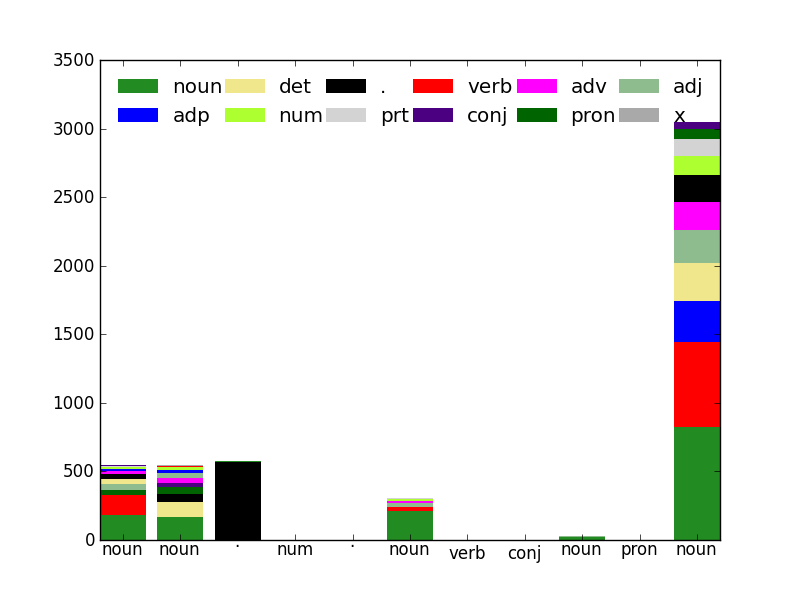
\includegraphics[scale=.5]{figs/sequences/cm_uns1.png}
\caption{\label{fig:cm_uns} Confusion Matrix example. Each cluster is a column. The best tag in each column is represented under the column (1-many) mapping. Each color represents a true Pos Tag.}
\end{figure}


\begin{exercise}
Run 20 epochs of the EM algorithm for part of speech induction:
\begin{python}
>>> hmm.train_EM(train_seq, 0.1, 20, evaluate=True)
>>> viterbi_pred_test = hmm.viterbi_decode_corpus(test_seq)
>>> posterior_pred_test = hmm.posterior_decode_corpus(test_seq)
>>> eval_viterbi_test =   hmm.evaluate_corpus(test_seq, viterbi_pred_test)
>>> eval_posterior_test = hmm.evaluate_corpus(test_seq, posterior_pred_test)

Initial accuracy: 0.303638
Iter: 1 Log Likelihood: -101824.763927
Iter: 1 Accuracy: 0.305441
Iter: 2 Log Likelihood: -78057.108346
Iter: 2 Accuracy: 0.321976
Iter: 3 Log Likelihood: -77813.725501
Iter: 3 Accuracy: 0.357451
Iter: 4 Log Likelihood: -77192.947674
Iter: 4 Accuracy: 0.385109
Iter: 5 Log Likelihood: -76191.800849
Iter: 5 Accuracy: 0.392123
Iter: 6 Log Likelihood: -75242.572729
Iter: 6 Accuracy: 0.391121
Iter: 7 Log Likelihood: -74392.892496
Iter: 7 Accuracy: 0.404249
Iter: 8 Log Likelihood: -73357.542833
Iter: 8 Accuracy: 0.399940
Iter: 9 Log Likelihood: -72135.182778
Iter: 9 Accuracy: 0.399238
Iter: 10 Log Likelihood: -70924.246230
Iter: 10 Accuracy: 0.395430
Iter: 11 Log Likelihood: -69906.561800
Iter: 11 Accuracy: 0.394328
Iter: 12 Log Likelihood: -69140.228623
Iter: 12 Accuracy: 0.390821
Iter: 13 Log Likelihood: -68541.416423
Iter: 13 Accuracy: 0.391522
Iter: 14 Log Likelihood: -68053.456865
Iter: 14 Accuracy: 0.389117
Iter: 15 Log Likelihood: -67667.318961
Iter: 15 Accuracy: 0.386411
Iter: 16 Log Likelihood: -67337.685686
Iter: 16 Accuracy: 0.385409
Iter: 17 Log Likelihood: -67054.571821
Iter: 17 Accuracy: 0.385409
Iter: 18 Log Likelihood: -66769.973881
Iter: 18 Accuracy: 0.385409
Iter: 19 Log Likelihood: -66442.608458
Iter: 19 Accuracy: 0.385409

>>> confusion_matrix = cm.build_confusion_matrix(test_seq.seq_list, viterbi_pred_test, 
                                             len(corpus.tag_dict), hmm.get_num_states())
>>> cm.plot_confusion_bar_graph(confusion_matrix, corpus.tag_dict, 
                            xrange(hmm.get_num_states()), 'Confusion matrix')
\end{python}
Note: your results may not be the same as in this example since we are using a random start, but the trend should be the same, with likelihood decreasing at every iteration (\textbf{the values in the example are the log likelihood, or the negative log likelihood? if it is the first, it is actually increasing}). 
%Also note that in some iterations the likelihood does not go down because of some rounding errors, however the general trend is that likelihood decreases over iterations. 
\end{exercise}

In the previous exercise we used an HMM to do Part-of-Speech induction using 12 clusters (by omission the HMM uses as number of hidden states the one provided by the corpus). A first observation is that the log-likelihood is always increasing as expected. Another observation is that the accuracy goes up from 33\% to 41\%. 
\todo{no exemplo e de 30.4\% a 38.5\%}
Note that normally you will run this algorithm for 200 iterations, we stopped earlier for time constraints. Another observation is that the accuracy is not monotonic increasing, this is because the likelihood is not a perfect proxy for the accuracy. In fact all that the likelihood is measuring are co-occurrences of words in the corpus; it has no idea of pos tags. The fact that we are improving derives from the fact that language is not random but follows some specific hidden patterns. In fact this patterns are what true pos-tags try to capture. A final observation is that the performance is really bad compared to the supervised scenario, so there is a lot of space for improvement. The actual state of the art is around 71\% for fully unsupervised~\citep{JoaoThesis,bergkirkpatrick2010naacl} and 80\% \citep{das-petrov:2011:ACL-HLT2011} using parallel data and information from labels in the other language. 

Looking at Figure \ref{fig:cm_uns}, it shows the confusion matrix for this particular example. 
A first observation is that most clusters are mapped to nouns, verbs or punctuation. 
This is a known fact since there are many more nouns and verbs than any other tags. Since maximum likelihood prefers probabilities 
to be uniform (imagine two parameters: in one setting both have value 0.5 so the likelihood will be 0.5*0.5 = 0.25, 
while in the other case one as 0.1 and 0.9 so the maximum likelihood is 0.09). Several approaches have been proposed to 
address this problem, moving towards a Bayesian setting \citep{johnson2007dtf}, or using 
Posterior Regularization \citep{graca2009nips}. 
%more about this later today. 
%Part-of-Speech induction is a very active field of research, in fact in the last two ACL conferences (Association for Computational Linguistics) the short paper award (2010) and the best paper award (2011) were about this topic~\citep{lamar-EtAl:2010:Short,das-petrov:2011:ACL-HLT2011}.








% \begin{exercise}

% Repeat the previous exercise using a different number of hidden states (20,50). Note that the higher the number of states is the slower the training will be.
% What do you observe? Look at the confusion matrix and try to explaing what is happening.

% \begin{python}
% In []: run readers/pos_corpus.py
% In []: posc = PostagCorpus("en",max_sent_len=15,train_sents=1000,dev_sents=0,test_sents=0)
% In []: run sequences/hmm.py
% In []: hmm = HMM(posc,nr_states=20)
% In []: hmm.initialize_radom()
% In []: run sequences/em.py
% In []: em = EM(posc,hmm)
% In []: em.train(posc.train,nr_iter=20)
% Init acc 0.348933
% Iter: 1 Negative Log Likelihood 16.038424
% Iter: 1 acc 0.362662
% Iter: 2 Negative Log Likelihood 11.200816
% Iter: 2 acc 0.370177
% Iter: 3 Negative Log Likelihood 11.046597
% Iter: 3 acc 0.380800
% Iter: 4 Negative Log Likelihood 10.607496
% Iter: 4 acc 0.389518
% Iter: 5 Negative Log Likelihood 9.809817
% Iter: 5 acc 0.394027
% Iter: 6 Negative Log Likelihood 8.949717
% Iter: 6 acc 0.396733
% Iter: 7 Negative Log Likelihood 8.105404
% Iter: 7 acc 0.398337
% Iter: 8 Negative Log Likelihood 7.366612
% Iter: 8 acc 0.392925
% Iter: 9 Negative Log Likelihood 7.005009
% Iter: 9 acc 0.393126
% Iter: 10 Negative Log Likelihood 6.895723
% Iter: 10 acc 0.397034
% Iter: 11 Negative Log Likelihood 6.851836
% Iter: 11 acc 0.397134
% Iter: 12 Negative Log Likelihood 6.818365
% Iter: 12 acc 0.399238
% Iter: 13 Negative Log Likelihood 6.782213
% Iter: 13 acc 0.406053
% Iter: 14 Negative Log Likelihood 6.755121
% Iter: 15 Negative Log Likelihood 6.745873
% Iter: 15 acc 0.419681
% Iter: 16 Negative Log Likelihood 6.743681
% Iter: 16 acc 0.424291
% Iter: 17 Negative Log Likelihood 6.745030
% Iter: 17 acc 0.431406
% Iter: 18 Negative Log Likelihood 6.747628
% Iter: 18 acc 0.434512
% Iter: 19 Negative Log Likelihood 6.749084
% Iter: 19 acc 0.438721
% pred = hmm.viterbi_decode_corpus(posc.train.seq_list)
% cm = build_confusion_matrix(posc.train.seq_list,pred,len(posc.int_to_pos),hmm.nr_states)
% plot_confusion_bar_graph(cm,posc.int_to_pos,range(12),"test")
% \end{python}

% \end{exercise}

%%% Local Variables: 
%%% mode: latex
%%% TeX-master: "../../guide"
%%% End: 




%%% Local Variables: 
%%% mode: latex
%%% TeX-master: "../../guide"
%%% End: 
